\title{Reading List}
\author{
        Mihaela Apetroaie-Cristea \\
        University of Southampton\\
         \underline{Southampton}
}
\date{\today}

\documentclass[12pt]{article}
\usepackage{graphicx}
\graphicspath{ {images/} }


\begin{document}
\maketitle

\section {Introduction to IoT}
\paragraph {Definition} Internet of Things (IoT, sometimes Internet of Everything) is the network of physical objects or "things" embedded with electronics, software, sensors and connectivity to enable it to achieve greater value and service by exchanging data with the manufacturer, operator and/or other connected devices. Each thing is uniquely identifiable through its embedded computing system but is able to interoperate within the existing Internet infrastructure \cite{wiki}.

\begin{figure}
\caption{Internet of Things Illustration}
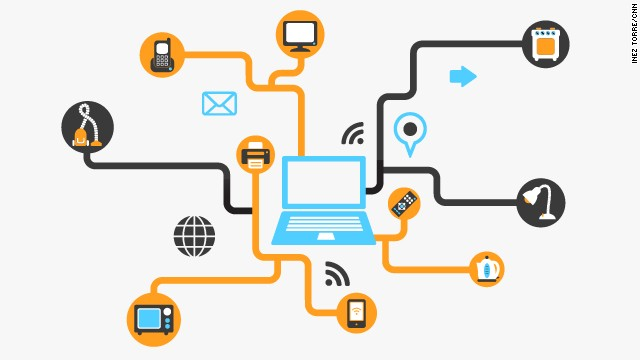
\includegraphics{iot}

\end{figure}

\paragraph {IoT desired characteristics}
\begin{enumerate}
\item\ \textbf {Automation:} Automation is a key feature of any IoT
device and application. Autonomous data collection, processing,
contextual inference, collaborating with other
IoT objects, and decision-making should be supported by
any IoT infrastructure.
\item\ \textbf {Intelligence:} Objects in IoT should act intelligently.
Building intelligence into these objects and empowering
them to operate adaptively based on different situations
is an important aspect. Situation and context awareness
are the key entities for an intelligent system, which can
operate with minimal human intervention.
\item\ \textbf {Dynamicity:} An object in an IoT ecosystem can move
from one place to another place. The IoT ecosystem
should be able to dynamically recognize and adapt these
objects based on the environment. Thus, dynamic management
and integration of these objects across different
environments and applications is crucial for a unified IoT
architecture.
\item\ \textbf {Zero configurations:} To support easy integration of
devices in the IoT ecosystem, plug-and-play feature
should be available. Zero-configuration support encourages
an easy and decentralized growth of IoT systems [4].
\end{enumerate}

\section{Internet of Things International Conferences}


\subsection {IoT 2015 Conference}
The 5th International Conference on the Internet of Things (IoT 2015) 


\paragraph{When and Where} October 26 - 28, 2015 in Seoul, S. Korea.

 \paragraph{Theme}The Internet of Things Conference is seeking original, high impact research papers on all topics related to the development of the Internet of Things. Papers will be reviewed and selected based on technical novelty, integrity of the analysis and social impacts and practical relevance.

\paragraph{Submission Deadline}
\begin{enumerate}
\item\ Abstract Registration: May 22, 2015
\item\ Paper Submission: June 4, 2015
\item\ Acceptance notice: July 31, 2015

\end{enumerate}

\subsection {HealthyIoT 2015 (IoT360) }
\paragraph {When and where}
\paragraph {Submission deadline} 30th June 2015
\paragraph {Theme} Internet of Things and Healthcare - electronic healthcare, patient care and medical data management.

\subsection {CoIoT (IoT360)} 2nd International Conference on Cognitive Internet of Things Technologies
\paragraph {When and where}  October 26 – 27, 2015 Rome, Italy
\paragraph {Theme} Cognitive IoT aims at gathering enthusiastic researchers and practitioners from AI and IoT-related areas sharing the common goal of addressing the new challenges posed by the Cognitive aspect of IoT, by using new or leveraging existing Artificial Intelligence techniques.

\paragraph {Submission deadline}
\begin{enumerate}
\item\ Full Paper Submission deadline: July 1, 2015
\item\ PCamera-ready deadline: August 25, 2015
\item\ Start of Conference: October 26, 2015
\item\ End of Conference: October 25, 2015
\end{enumerate}

\subsection{FiCloud 2015 } The 3rd International Conference on Future Internet of Things and Cloud
\paragraph {When and where} Aug 24, 2015 - Aug 26, 2015, Rome, Italy
\paragraph {Theme} The theme of this conference is to promote the state of the art in scientific and practical research of the IoT and cloud computing. It provides a forum for bringing together researchers and practitioners from academia, industry, and public sector in an effort to present their research work and share research and development ideas in the area of IoT and cloud computing. 
\paragraph {Submission Deadlines} 
\begin{enumerate}

\item\ Submission Deadline:	Apr 16, 2015
\item\ Notification Due	May: 30, 2015
\item\ Final Version Due: Jun 20, 2015
\end{enumerate}
\subsection{IEEE on Internet of Things} 
\paragraph {When and where} 14 - 16th December 2015 Milan, Italy
\paragraph {Theme} The 2015 IEEE 2nd World Forum on Internet of Things (WF-IoT) - Technologies, Applications and Social Implications is a unique event for industry leaders, academics and decision making government officials. This event is designed to examine key critical innovations across technologies which will alter the research and application space of the future. The Internet of Things envisions a highly networked future, where every object is integrated to interact with each other, allowing for communications between objects, as well as between humans and objects, which enables the control of intelligent systems in our daily lives.
\paragraph {Deadlines}
\begin{enumerate}
\item\ Submission deadline: 8th July 2015
\item\ Acceptance notification: 15th September 2015

\end{enumerate}

\subsection {RFID Journal Introduces Internet of Things Conference}
\paragraph {When and where} Apr. 16-17 2015, in San Diego, Calif.
\paragraph {Theme} Anything IoT related.

\section{Internet of Things Interesting Projects}

\subsection{Health system - information related} An application for Health System that will allow everyone see relevant information about the patients depending on whom is accessing it.
\paragraph {} "If I am a doctor, I should have access to a patient's health records. If I'm the guy who needs to clean the bedpan, all I need to know is when I need to go in and clean a room." Using District Defend, mobile devices could deliver data based on who is using the tablet and where he or she is located.

 \subsection{Inteligitics} Uses temperature, humidity and light sensors that transmit data via ZigBee and Bluetooth transceivers to help logistics companies monitor the condition of fruits and vegetables in transit, in order to keep them in optimal conditions and extend shelf life \cite{notes}.

  \subsection {Olea Sensor Networks} It is a Sunnyvale, Calif.-based startup, introduced its sensor platform, made to enable end users to differentiate animate from inanimate objects—and even to determine whether animate objects are human or non-human -  NASA uses somehting similar to find individuals for disaster and emergency response (FINDER)\cite{olea}.

\subsection {Soundhawk's application} It reduces the ambient noise so that, for example, if you are in a crowded pub you can enjoy the conversation at your table by minimising the background noise.

 \subsection {Aquarium app for visitors} It sends alerts via an app when the phone is in the range of any of the beacons they mounted. It helps kids actively learn about the species within the aquarium -  has been used for The Tennessee Aquarium, in Chattanooga \cite{norman}

\subsection {Wifi Smart Pen: Sky}
A pen that will sync what you write a paper on electronic devices i.e tablet, phone and so on - it will virtually reproduce your notebook \cite {pen}.  One downside of the system is you are required to use a proprietary Livescribe dot notebook (free with a pen purchase) in order for the full optical character recognition (OCR) of your handwriting to be read, searched and played back to you in a "pencast".
\subsection {Home Energy Monitor: Hyko Bear} A device, in shape of a bear, that changes its colour when with the energy usage \cite{bear}. 

\paragraph {How does the bear know what’s going on with the electrical system?} A wireless sensor, of course! The device comes with a small box that clamps to the main cable near a home’s energy meter. Data on the current flowing into the house is transmitted by an 868 Mhz radio, which is also used by other building infrastructure monitors such as some thermostats and fire alarms.
\subsection {Sensor Sleep Shirts: RestDevices} A shirt that can monitor your quality of sleeping or can be used for babies. It provides parents with information around their child's skin temperature, body position, and respiration and can alert them if something unusual is detected \cite{shirt}.
\subsection {Golf Glove Sensors: GolfSense}  Golf glove that monitors your movements during the game. They want to also include the option when you are allowed to compare your movement with others \cite{golf}. 

\subsection {mCookie} Hardware compatible with lego \cite{lego}
\subsection {Wi-Fi Indoor Air Quality Sensor: Foobot}

A device that that measures carbon dioxide, carbon monoxide, volatile organic compounds, particulate matter, temperature and humidity. In time it will be able to make correlations between bad habbits and air quality and help improve the air quality in homes \cite{air}.
\begin{figure}
\caption{User Interface for Footbot}
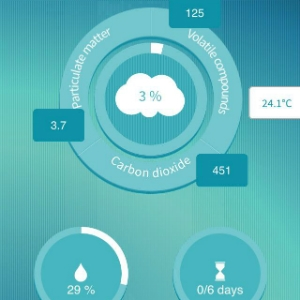
\includegraphics{ai}

\end{figure}

 \section {List with harware}

\begin{enumerate}
\item\ compass
\item\ gyroscope 
\item\ accelerometers
\item\ micro-controller

\end{enumerate}

 \bibliographystyle{abbrv}
 \bibliography{main}
 \begin{thebibliography}{1}
 \bibitem {wiki} Wikipedia \emph{https://en.wikipedia.org/wiki/Internet_of_Things}
 \bibitem {ieee} Chayan Sarkar \emph{DIAT A Scalable Distributed Architecture for IoT} IEEE INTERNET OF THINGS JOURNAL, VOL. 2, NO. 3, JUNE 2015.
 \bibitem {notes} IoT Journal \emph{http://www.iotjournal.com/articles/view?13044} 2015
 \bibitem {olea} IoT Journal \emph {http://www.iotjournalcom/articles/view?13016} 2015.
 \bibitem{norman} IoT Journal \emph{http://www.iotjournal.com/articles/view?12851} 
 \bibitem {pen} Wifi Smart Pen: Sky \emph{http://postscapes.com/wifi-smart-pen-sky} 
 \bibitem{bear} Postscapes \emph{http://postscapes.com/home-energy-monitor-hyko-bear}
 \bibitem{shirt} Postscapes \emph{http://postscapes.com/sensor-sleep-shirts-restdevices}
 \bibitem{golf} postscapes \emph {http://postscapes.com/golf-glove-sensors-golfsense}
 \bibitem{lego} Postscapes \emph {http://postscapes.com/lego-compatible-prototyping-kit-mcookie}
 \bibitem{air} Postscapes \emph{http://postscapes.com/wi-fi-indoor-air-quality-sensor-foobot}

 \end{thebibliography}
\end{document}

  